\documentclass{article}

\usepackage{graphicx}
\usepackage{subcaption}
\usepackage[margin=1in]{geometry}			%margins
\usepackage{indentfirst}					%indentation
\usepackage{listings}						%code
\usepackage{hyperref}
\usepackage{color}

\setlength{\intextsep}{15pt plus 1.0pt minus 2.0pt}		%figure spacing inside text

\begin{document}

\title{Sketch-to-Spice converter: Installation guide}
\author{Tarek Tohme}
\date{May 7th, 2018}
\maketitle


\section{Step 1: Downloading and installing OpenCV}
Sketch-to-Spice requires OpenCV to run. Here are links to tutorials on how to install it for linux and Mac.

\paragraph{Linux}
Follow this \href{https://docs.opencv.org/2.4/doc/tutorials/introduction/linux_install/linux_install.html}{\color{blue}link}

\paragraph{Mac}
If you have homebrew, you can run the following command:

brew install opencv

from the terminal.

if not, you can install it by following this \href{http://osxdaily.com/2018/03/07/how-install-homebrew-mac-os/}{\color{blue}tutorial}.

\section{Step 2: Using the binary}
After unzipping the Sketch-to-Spice folder, you can run the program from the terminal window
using ./symboldetector.

\section{Step 3: Building the binary from source code (optional)}
An easy way to build the binary from the cpp files is to use CMake. If you don't have it installed, you can get it from the \href{https://cmake.org/download/}{\color{blue}CMake download page} .

After setting up CMake and OpenCV, create a text file called CMakeLists.txt, with the following contents (replacing the name of the executable and with symboldetector)

% Figure 1: CMakeLists contents
\begin{figure}[h]				%placement (here)
	\centering
	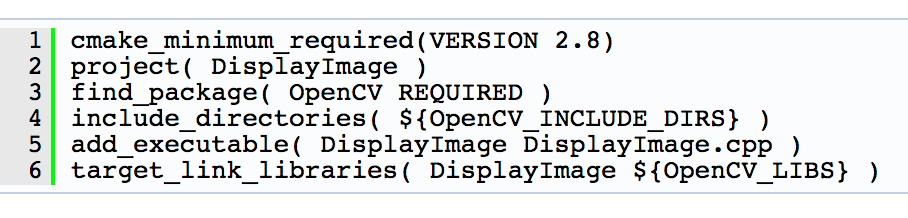
\includegraphics[width=11cm]{cmakepic}
\end{figure}

To generate the executable, just run the following commands:

% Figure 1: Generate executable
\begin{figure}[h]				%placement (here)
	\centering
	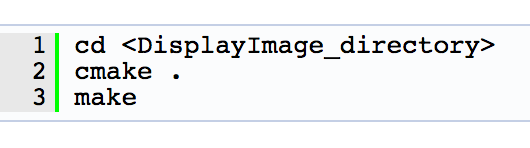
\includegraphics[width=6cm]{genexec}
\end{figure}

\section{Training your own classifier}
\href{https://docs.opencv.org/3.1.0/dc/d88/tutorial_traincascade.html}{\color{blue}This link} shows you how to train your own cascade classifier. I wrote a tool that simplifies the process of generating training images. You can find it in the classifier folder, under the name extractimages. The binary can be built and run by following the same steps as for the symboldetector.

Here's how to use it:
\begin{itemize}
\item Draw about 150 symbols of the component you wan to train the classifier for on a piece of A4 paper.
\item Scan the paper
\item run extractimages with the path of the scanned image as the first argument on the command line, and the name of the component as the second argument. For example:
\end{itemize}

% Figure 1: Generate executable
\begin{figure}[h]				%placement (here)
	\centering
	
\includegraphics[width=12cm]{extimg}
\end{figure}


You should see a folder containing cropped binary images of each component drawn on the paper. The tool also produces the info file and a file containing the paths to the images, which are used in the tutorial to train the classifier. You can also use the tool to produce the negatives, or background images mentioned in the tutorial.

\paragraph{}
After training a classifier, you can input the path of the cascade.xml file to the application to enable detection for more components. Read the Help paragraph in the application for more info. You can use the following recommended settings to train the classifier:

-numPos 140

-numNeg 600

-numStages 5

-w 100

-h 25

-maxFalseAlarmRate 0.1

\section{Try it out!}
We suggest you try the application out with the test5.jpeg image, located in the test\_set folder. The object detector is quite sensitive to lighting, and it was trained using the author's own style of drawing, so getting it to detect other styles of components might be tricky. Also, it can only detect resistors, as this is a free trial version.


\end	{document}